% !TEX root =  ../master.tex
\chapter{Konzeption}
Bevor mit der Implementierung gestartet werden kann wird ein Konzept erstellt, welches als Leitfaden für die Implementierung dienen soll.
Ziel ist es ein Entwurf zu konkretisieren, welcher die technischen und grundlegenden Funktionalitäten beschreibt.
Dadurch soll verhindert werden, dass die aufwendige Implementierung fehlschlägt oder mehrfach Änderungen durchgeführt werden müssen, welche den Implementierungsaufwand vergrößern würden.

% TODO: Wasserfall / Agile

\section{Konzeption der Anwendungsarchitektur}

\subsection{Infrastruktur}
Die Grundlage jeder Anwendung ist der Aufbau und die Struktur der Infrastruktur, auf welcher die Anwendung später ausgeführt werden soll.
Aus diesem Grund wird diese als erstes betrachtet.

Webanwendungen werden üblicherweise in einem Client-Server-Modell entwickelt.
% TODO: \autocite{Leff}
Der Client übernimmt dabei sämtliche Funktionalitäten, die das Nutzerinterface betreffen.
Dazu zählt die Visualisierung und die Interaktion mit dem Nutzer.
Der Server kümmert sich hingegen um die Geschäftslogik, Datenhaltung und Datenaustausch.
In \autoref{fig:clientServerAufbau} ist eine solche Architektur vereinfacht dargestellt.

% TODO: Thin-Client

\begin{figure}[h]
    \centering
    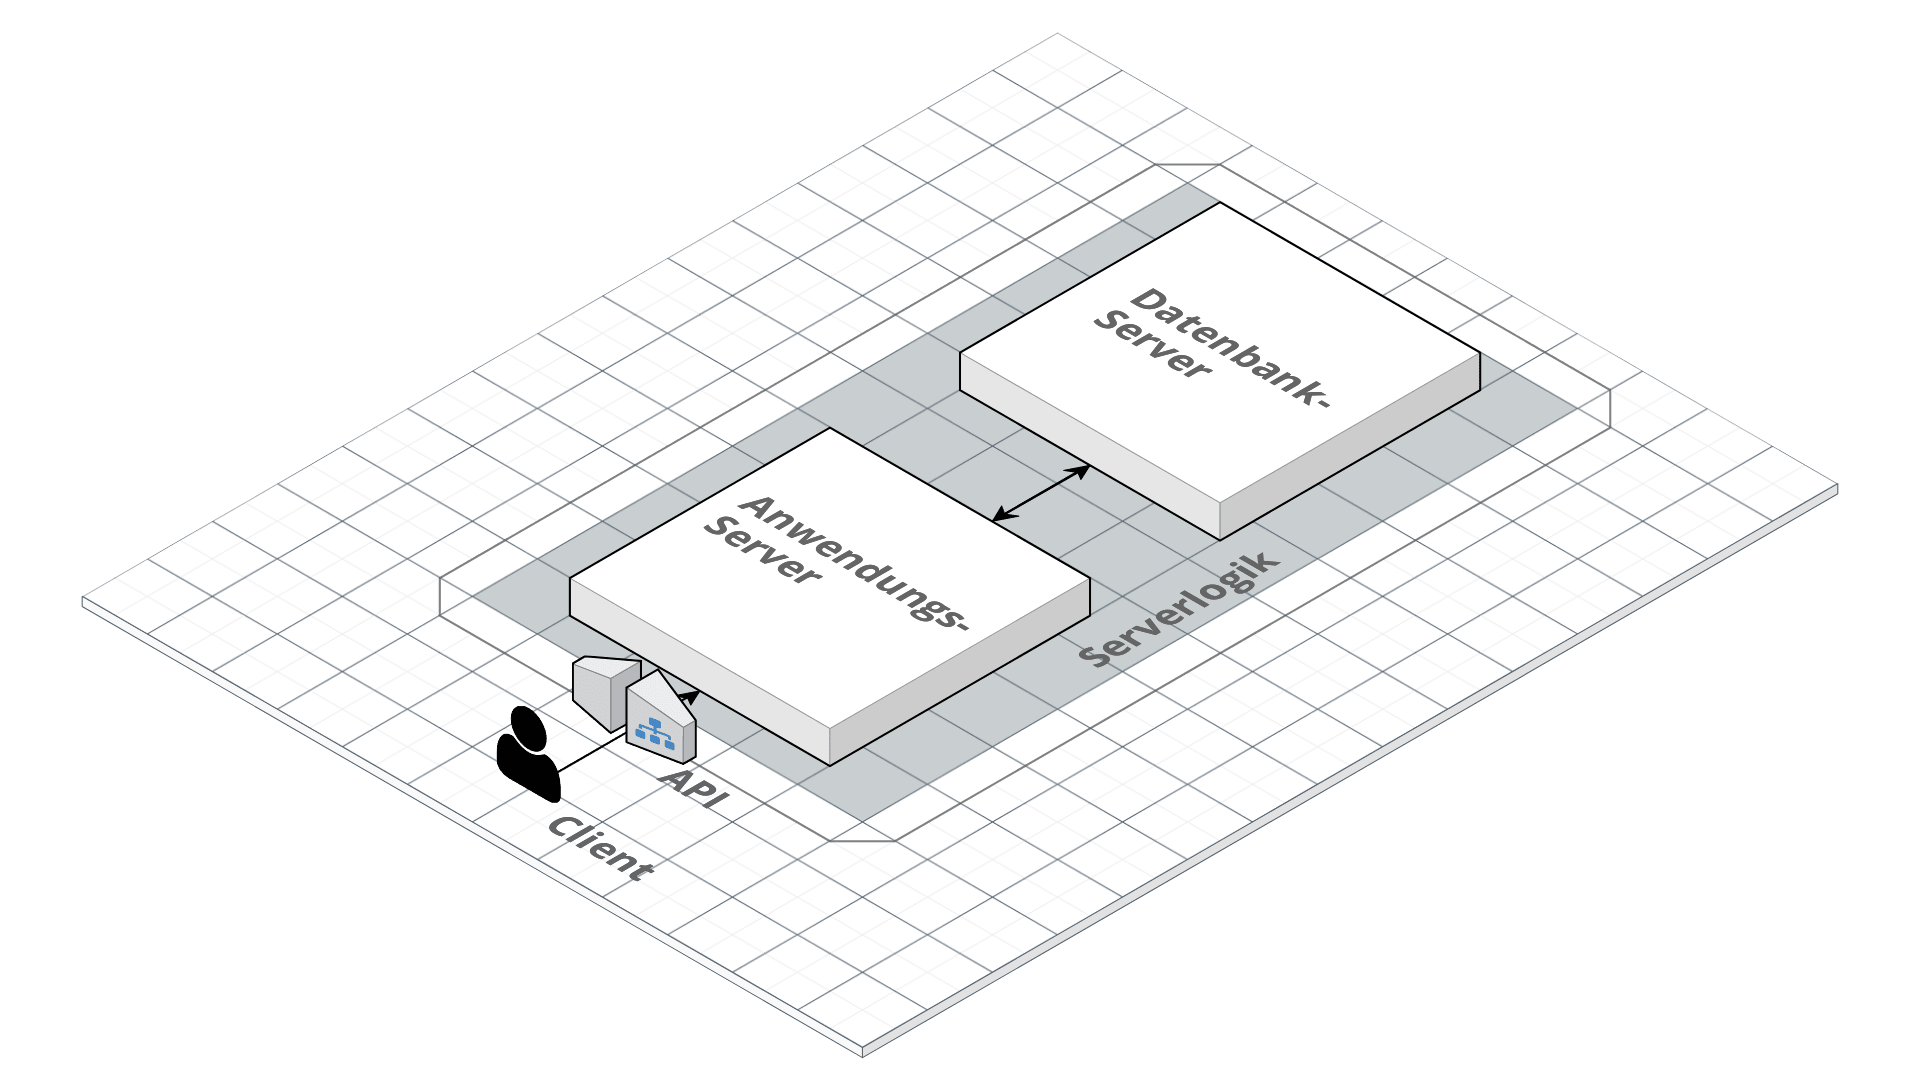
\includegraphics[width=.9\textwidth]{img/ClientServer.png}
    \caption{Vereinfachter Client-Server-Aufbau}
    \label{fig:clientServerAufbau}
\end{figure}

Der Nutzer ruft die mithilfe seines Browsers die Webseite von einem Server ab.
Frägt der Nutzer und in seiner Verlängerung der Browser Daten an, werden diese vom Anwendungsserver geladen.
Dabei greift der Nutzer über eine \ac{API} auf den Anwendungsserver zu.
Dieser läd die notwendigen Informationen auf ähnliche Weise von einem Datenbankserver und bereitet diese gegebenenfalls auf.

Nach den Anforderungen ist eine hohe Leistungsfähigkeit benötigt wird, die auch mit Leistungsspitzen klar kommt.
Der Nachteil von Client-Server-Modellen ist der hohe Aufwand im Bereich der Skalierung.
Das heißt, sobald eine Leistungsspitze entsteht müssen erst aufwändig zusätzliche Server hochgefahren werden, welches die Anwendung kurzzeitig für viele Nutzer unnutzbar macht.
Aus diesem Grund haben wir uns für einen modernen \enquote{Serverless}-Ansatz entschieden.

% TODO: Cloud Computing

% TODO: Serverless Computing
% TODO: Das vielleicht in Grundlagen verschieben
% TODO: Hier kann man noch super viel schreiben

% TODO: Hier noch vielmehr schreiben wie Nutzenanalyse? + viel überleitung


\begin{figure}[h]
    \centering
    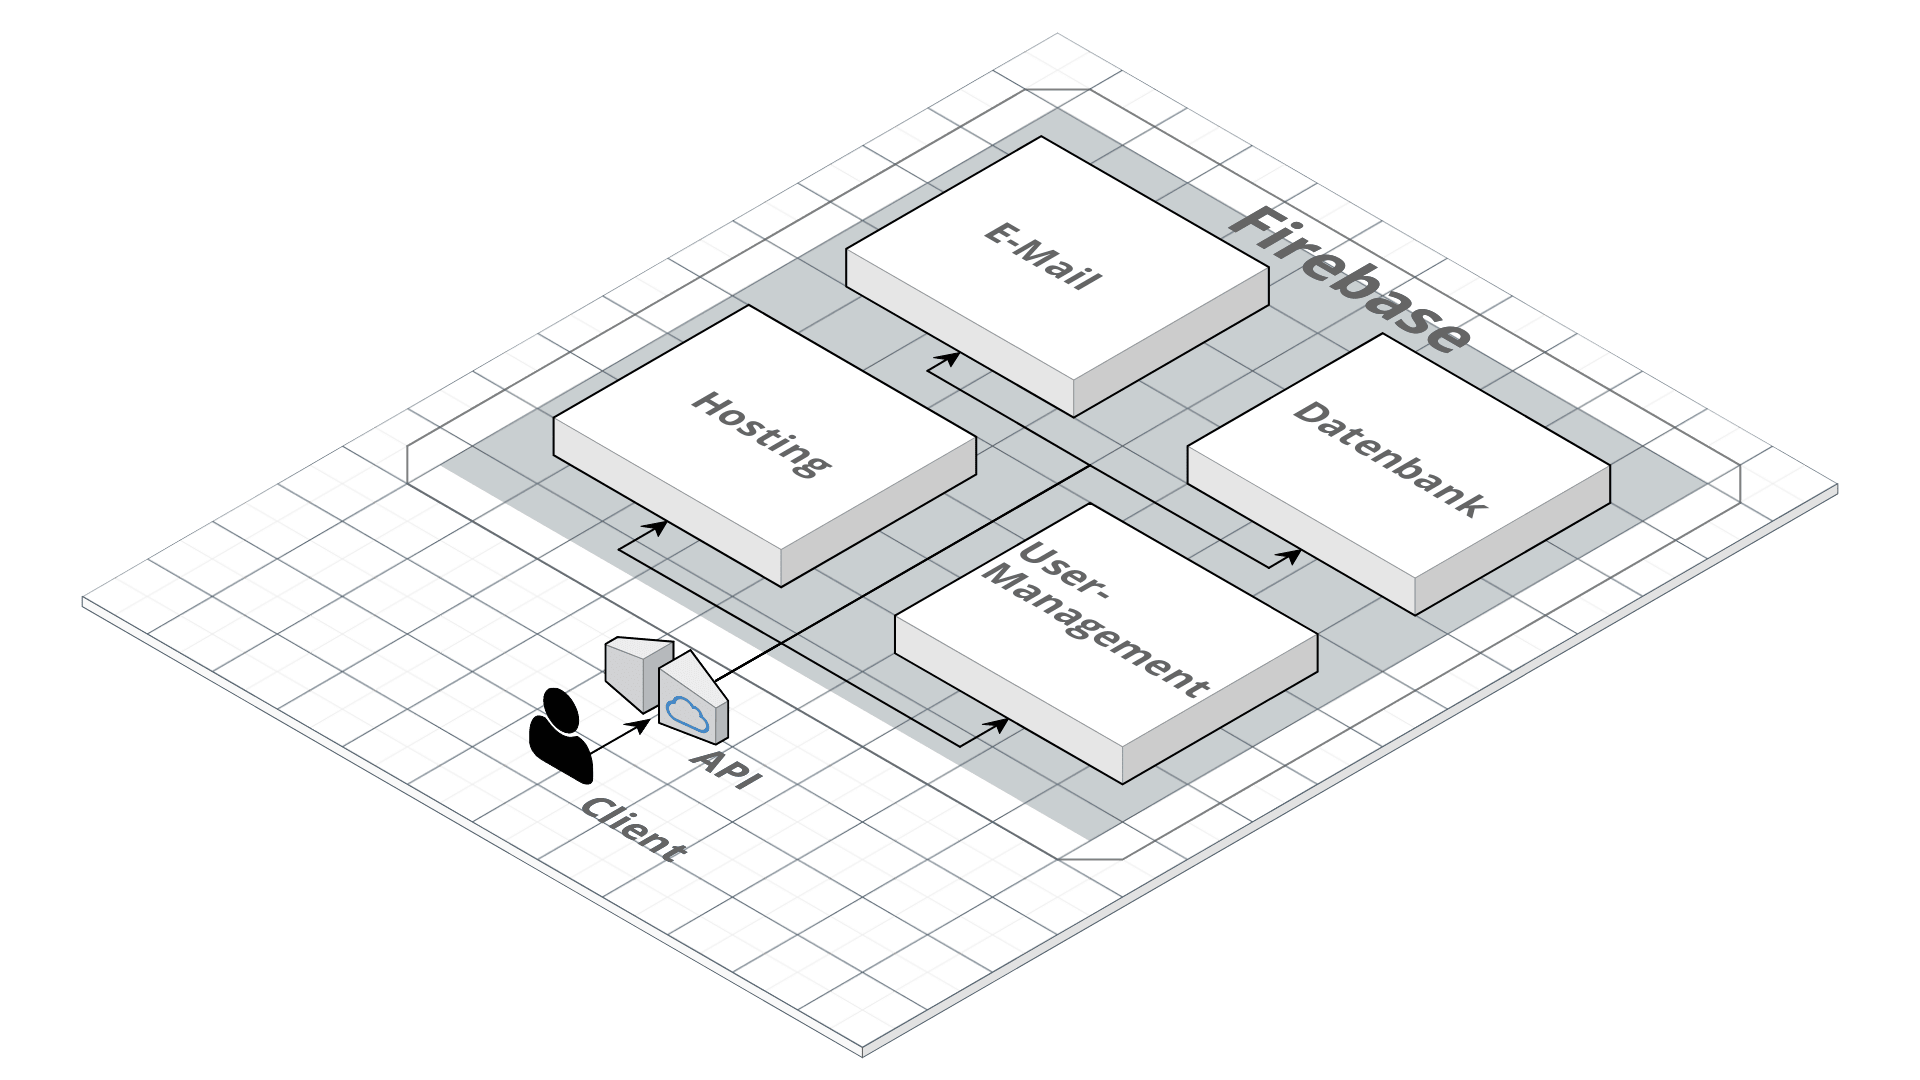
\includegraphics[width=.9\textwidth]{img/Firebase.png}
    \caption{Vereinfachter Firebase-Aufbau}
    \label{fig:firebaseAufbau}
\end{figure}



\subsection{Anwendungsaufbau}
Für das Nutzerinterface werden verschiedene Technologien verwendet.




\section{Konzeption der Funktionalitäten}


\subsection{Kurseinschreibung} %TODO: F2,   das hier vielleicht mit Rollenzuweisung tauschen von der Reihenfolge
Aus den Anforderungen geht hervor, dass es zwei Nutzerrollen gibt: Dozenten und Studenten.
Dozenten sollen in der Anwendung ihre Kurse verwalten können.
Ein Kurs orientiert sich dabei an der Organisation, die in der Realität vorliegen.
Auch in vorhandenen Tools wie beispielsweise \enquote{Moodle} sind Studenten anhand von Kursen organisiert.
Aufgrund der Vielzahl an solchen Lösungen scheint sich eine solche Organisation zu bewähren.
Aus diesem Grund liegt es nahe, das auch die zu entwickelnde Anwendung eine solche Struktur nutzen sollte.
% TODO: Wie Werden Kurse erstellt

Nachdem nun geklärt wurde, wie die Organisation von Studenten und Dozenten stattfindet, muss nun die Zuweisung von Studenten zu Kursen die Zuweisung von Dozenten konzipiert werden.
Zunächst wird die Studentenzuweisung betrachtet.
Für die Zuweisung von Studenten kommen mehrere Ansätze in betracht, die sich in der Person unterscheiden, die die Zuweisung durchführt:
\begin{enumerate}
    \item Zuweisung durch Anwendungsadministrator
    \item Zuweisung durch Dozenten
    \item Zuweisung durch Studenten
\end{enumerate}
Als erster Ansatz kommt die Zuweisung durch einen Anwendungsadministrator in betracht.
Ein solcher Administrator ist ein zentraler Mitarbeiter der DHBW, welcher komplette Autorität über die Anwendung besitzt.
Von einem solchen Ansatz wird abgesehen, da der Verwaltungsaufwand sehr hoch ausfällt.
Für jeden Kurs über 20 Studenten zuzuweisen, und das für mehrere Kurse pro Semester und Vorlesung, scheint nicht realistisch.

Der zweite ist der Ansatz der Zuweisung durch einen Dozenten.
In der aktuellen DHBW-Organisation besitzen Dozenten bereits eine Liste an Studenten für ihre Vorlesung.
Diese Liste dient zur Anwesendheitskontrolle.
Demnach können Dozenten diese Liste für die Zuweisung in der Anwendung nutzen.
Der Nachteil eines solchen Ansatzes ist es aber, dass Studenten ihre Daten in der Anwendung hinterlassen müssen und diese durch andere Dozenten gegebenenfalls einsehbar wären.
Zusätzlich geht die Anonymität, welche durch Matrikelnummern gegeben ist eventuell verloren.
Insgesamt ist dieser Ansatz aus Datenschutzaspekten besonders kritisch. % TODO: Beim Admin nicht so, weil dhbw

Als Letzter Ansatz ist die Zuweisung durch den Studenten.
Denkbar sind hier mehrere Ansätze: Eine Liste aus Kursen oder über einen Kursidentifikator.
Eine Liste mit Kursen vereinfacht die Zuweisung durch den Studenten, da Kurse schnell entdeckt werden können und eventuell zusätzliches Wissen vermittelt werden kann, wenn der Student sich für mehrere ähnliche Kurse einträgt.
Nachteil ist aber die unmittelbare Verwaltung und Übersicht über die Kurse.
Eine Zuweisung über einen Kursidentifikator (kurz: Schlüssel) hat den Nachteil, dass diese Schlüssel erst aufwändig über einen weiteren Kommunikationsweg (z.\,B. Email oder direkt in einer Vorlesung) mitgeteilt werden muss.
Dafür besitzen Studenten aber nur Zugriff auf die für sie relevanten Vorlesungen.
In \enquote{Moodle} ist die Zuweisung zu Kursen auf freiwilliger Basis anhand von Einschreibeschlüsseln gelöst.
Aus diesem Grund ist dieser \enquote{Workflow} bereits für Studenten bekannt und eine Anpassung an die neue Anwendung ist schnell möglich.
In der Tat nutzen viele existierende Anwendungen ein solches System.
Beispiele hierfür sind Zoom oder Google Meets.

% TODO: Bei uns:
Ein Einschreibeschlüssel besteht aus 6 Buchstaben, welche mehr als 300 Millionen Kurse zulassen und als ausreichend angesehen werden.


\subsection{Rollenzuweisung} %TODO: Nochmal auf die Anforderungen F7 verweisen
Nutzer der Anwendung können sich selbst registrieren.
Daraus ergibt sich die eine Rollen Problematik: Woran kann die Anwendung erkennen, welcher Nutzer ein Student ist und welcher Nutzer ein Dozent ist.
Sofern Nutzer dies selber angeben können, bräuchte es gegebenenfalls eine Validierung durch die DHBW, wodurch erneut die oben genannten Nachteile einer Zuweisung durch einen Administrator greifen.
Ein Ansatz, bei dem Nutzer dies selber verwalten können wird auch hier als besser angesehen.
Aus diesem Grund wird der folgende Ansatz verwendet:
Statt festdefinierte Rollen (Student und Dozent) zu besitzen, kann jeder Student selbst sowohl Student, als auch Dozent sein.

Jeder Nutzer ist zunächst keiner Rolle zugeordnet.
Jeder Nutzer kann einen Kurs erstellen, wodurch dieser Nutzer automatisch zu einem Dozent für diesen Kurse.
Sobald sich ein Nutzer mithilfe des Einschreibeschlüssels für einen Kurs anmeldet wird der Nutzer automatisch für diesen Kurs zu einem Studenten.
Dadurch können auch zuvor nicht vorgesehene Nutzerbeziehungen entstehen.
Beispielsweise kann ein Dozent sich in einen weiteren Kurs einschreiben, falls er sich in einer weiteren Richtung weiterbilden möchte.
Oder die DHBW kann sich in für einen Kurs einschreiben um die Qualität einer Vorlesung zu validieren.


Ein Vorteil eines solchen Ansatzes ist es, dass auch Studenten Kurse erstellen können und so Lerngruppen gefördert werden.
Denkbar ist beispielsweise ein Student, welcher Nachhilfe anbietet.
Dadurch wird die Nutzung der Anwendung gefördert.



% TODO: Mocks und alles

% \section{Frontendarchitektur}
% \section{Datenmodell und Datenhaltung}

% Die Anwendung folgt dem \ac{MVC}-Pattern. Das heißt, die Anwendung ist aufgeteilt in 3 Bereiche:
% \begin{itemize}%TODO: Hier kann man noch mehr schreiben
%     \item Model\\
%         Das Modell stellt den aktuellen Status bzw. den aktuellen Zustand der Anwendung dar.
%     \item View\\
%         Die Präsentation ist zuständig für die Darstellung der Daten und ermöglicht dem Benutzer die Interaktion mit diesen sowie die Steuerung der Anwendung.
%     \item Controller\\
%         Der Controller kümmert sich um die Steuerung der Anwendung. Er verwaltet die Präsentation und steuert den Datenfluss zwischen der Präsentation und dem Modell.
% \end{itemize}
% % \begin{wrapfigure}{r}{5.5cm}
% %     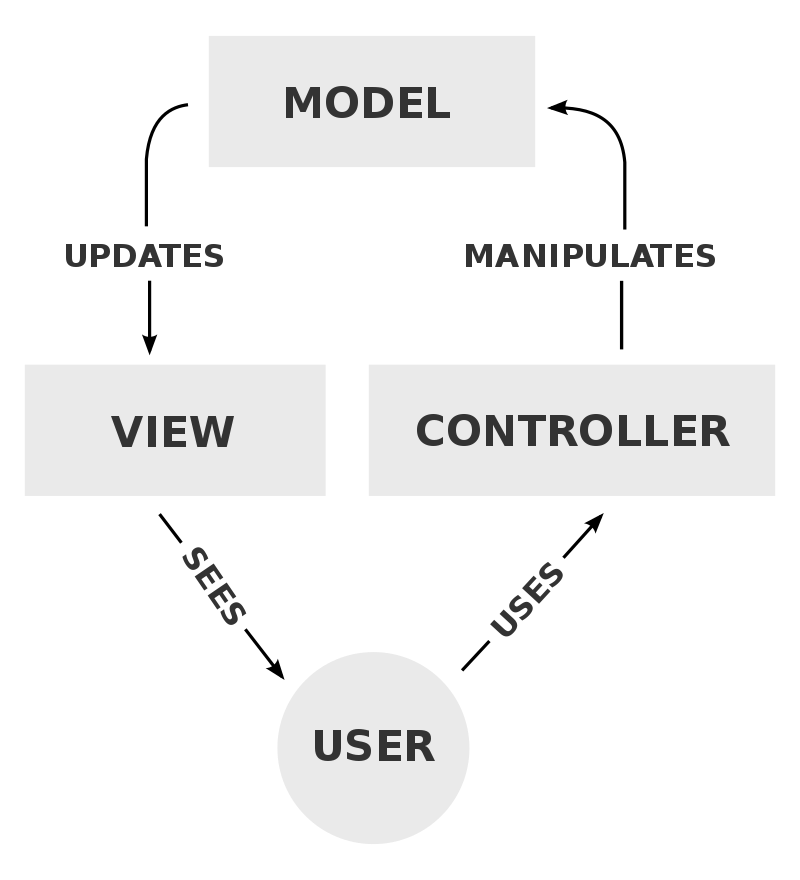
\includegraphics[width=.25\textwidth]{img/1024px-ModelViewControllerDiagram2.svg.png}
% %     \caption{}
% %     %TODO: https://en.wikipedia.org/wiki/Model%E2%80%93view%E2%80%93controller#/media/File:MVC-Process.svg
% %   \end{wrapfigure} 

% % TODO ER-Modell



% \subsection{Studierende}
% \subsection{Dozierende}
% \subsection{Kurs erstellen}
% \subsection{Karteikarten-Lernsystem}
% \subsection{ToDo-Liste}
% \section{Datensicherheit}
% \section{Datenschutz}
% \section{Grundlage für Datenauswertung}
% % Hier Verweise auf Aubau und Bezug zum leichten Ausbau, etc.








\section{Ich mach hier einen WIP Abschnitt :D}













% Authentifizierung
Damit die Zuweisung von Nutzern, Dozenten und eine nutzerspezifische Speicherung von Daten (z.\,B. Todos) möglich ist, wird eine Authentifizierung notwendig.



Bei der Entwicklung der Anwendung haben wir großen Wert auf Datensicherheit und der Einhaltung der DSGVO gelegt.
Ein wesentlicher Bestandteil der unternommenen Maßnahmen ist die Anonymität innerhalb der Anwendung.
Die Anwendung speichert keinerlei Informationen, worüber Nutzer identifiziert werden können.
Bei einer Registrierung muss lediglich eine Email angegeben werden.








% TODO: Das besser mit den Anforderungen verknüpfen
% TODO: Dokumentation über TODOS


% TODO: Todos und index-cards auch löschbar und alles

% TODO: Wie technisch?






% TODO: Dokumentation über Authentifizierung
% TODO: Dokumentation über Index-Cards
% TODO: Screenshots
% TODO: Aria?





% Ein Dozent sollte dabei beispielshaft einen Kurs anlegen können

Um eine möglichst gute Nutzererfahrungs zu ermöglichen wurden einige umfangreiche Maßnahmen ergriffen.



Bei der Entwicklung wurde auf die responsive Darstellung geachtet.
So verhalten sich alle Funktionalitäten einer Anwendung wie es von einer nativen Anwendung erwartet wird.
Dies macht sich besonders in der optimierten Darstellung bemerkbar, bei der der Nutzer nicht zu scrollen oder zoomen verpflichtet ist bemerkbar.
Aber auch andere Funktionalitäten, wie das Wischen der Karteikarten funktioniert auf Geräten mit einem Touchscreen genauso, wie auf Geräten, welche eine Maus verwenden. 


Die Anwendung unterstützt Code-Splitting mit Lazy-Loading.
Das bedeutet, die Anwendung ist modular aufgebaut und wird zum Zeitpunkt der Bereitstellung automatisch in verschiedene Module aufgespalten.
Besucht der Nutzer die Website der Anwendung werden nur die Teile der Anwendung heruntergeladen, die für ihn tatsächlich notwenig sind.
Beispielsweise werden die Karteikarten, sowie die gesamte Funktionalität und Darstellung dieser nicht geladen, wenn der Nutzer nur seine Todos nachschaut.


% TODO: Caching


% TODO: Lighthouse am schluss beschreiben, wenn wir alle unnötigen Abhängigkeiten entfernt haben?

% TODO: Kann man nach offline machen?

Der Ladefortschritt kann stets an der Leiste am oberen Bildschirmrand abgelesen werden.

